\chapter{Sviluppo ed Utilizzo}
\label{chapter:implementazione}

\section[Sistema Realizzato per Simulazioni ed Analisi]{Sistema Realizzato per Simulazioni ed\\ Analisi}
\label{section:sistema_analisi}

Al fine di valutare le prestazioni degli scenari di Fog Computing, descritti al Capitolo \ref{chapter:architettura}, è stato implementato un sistema di simulazione che ne permette in una prima fase la definizione (topologia, applicazioni, servizi, richieste, ecc...) e, successivamente, l'analisi dei principali aspetti utili alla comprensione dello scenario, come il successo del \textit{service placement} e delle richieste di servizi da parte dei nodi della rete.

La definizione e l'esecuzione della simulazione seguono il diagramma di flusso mostrato in Figura \ref{fig:sim_flow_diagram}. Tramite il software realizzato è possibile eseguire due principali tipologie di analisi:
\begin{enumerate}
	\item \textbf{analisi del service placement con cambio di parametri}: viene valutato il successo del service placement al variare di specifici parametri di definizione dello scenario, specificando il numero di iterazioni e quali di questi devono variare ad ogni esecuzione;
	\item \textbf{simulazione di uno scenario specifico}: una volta definito e simulato uno specifico scenario, è possibile ottenere un'analisi sul soddisfacimento delle richieste da parte dei nodi dei vari servizi offerti dalla rete, con e senza \textit{failure control} dei nodi.
\end{enumerate}


\begin{figure}[!ht]
  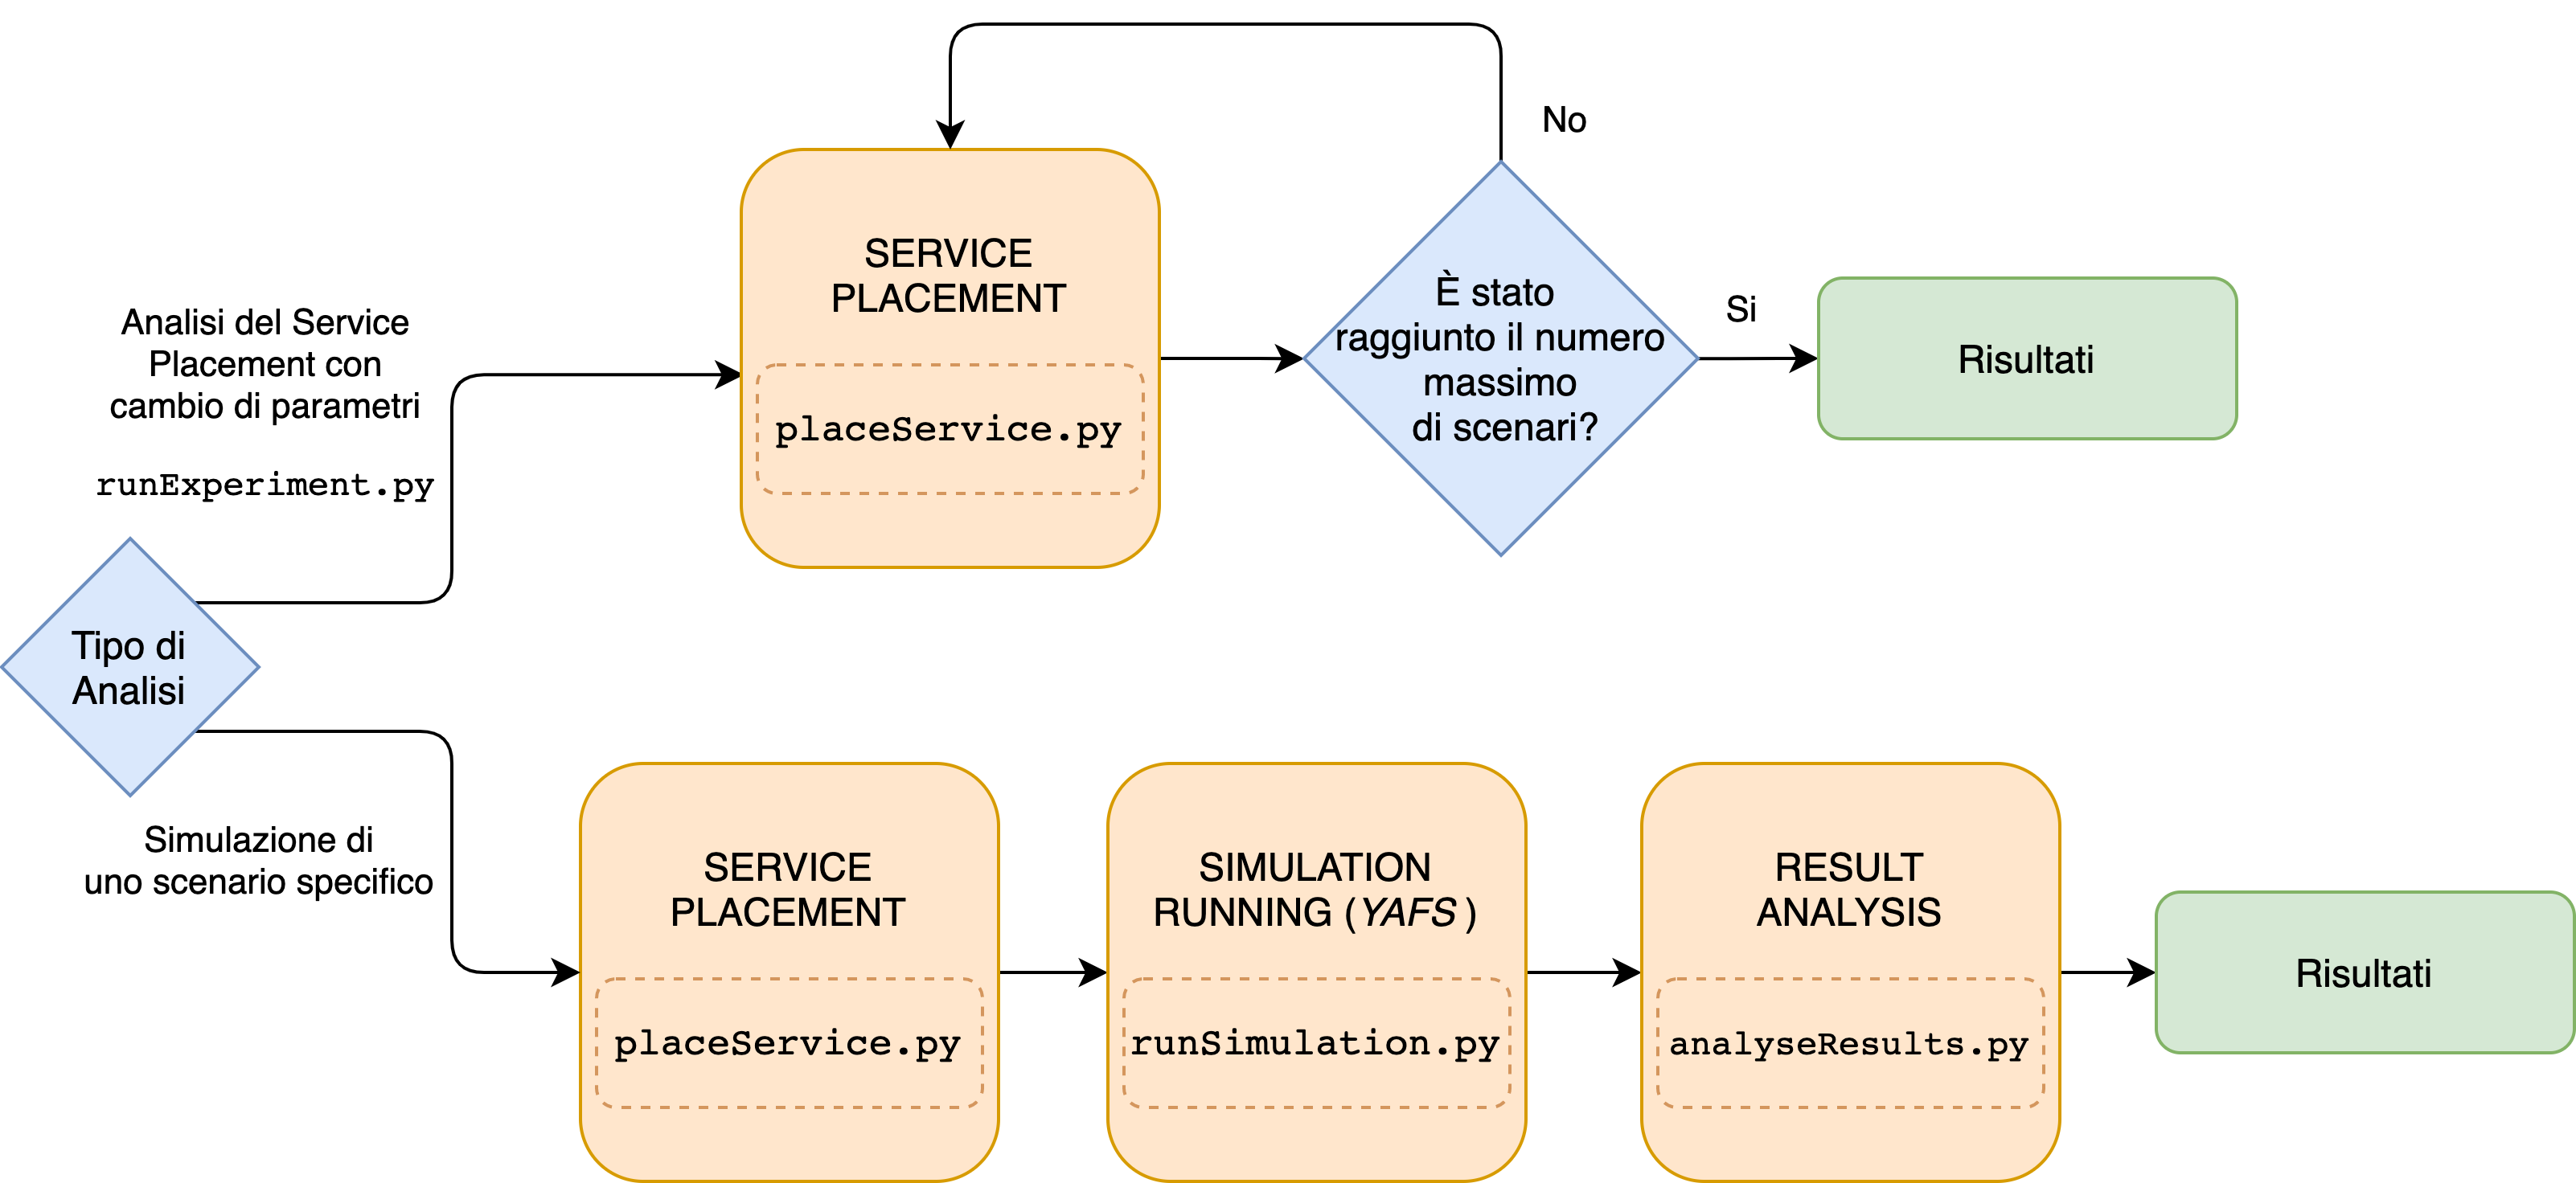
\includegraphics[width=14cm]{images/sim_flow_diagram}
  \centering
  \caption{Diagramma di flusso del sistema di simulazione.}
  \label{fig:sim_flow_diagram}
\end{figure}

\subsection{Utilizzo del Software Realizzato}

Entrambe le tipologie di simulazione prevedono alcuni passaggi obbligati. Nella fase di inizializzazione è necessaria la configurazione dell'esperimento. Questa può essere eseguita tramite opportune modifiche al file \texttt{\justify experimentConfiguration.py}. Le possibilità di configurazione sono esposte nel seguito.

\subsubsection{Configurazione della Topologia}

La topologia, generata dinamicamente in fase di inizializzazione, può essere configurata con i seguenti parametri:
\begin{itemize}
	\item \texttt{IOT\_DEVICES\_NUM}: il numero di device IoT che la rete deve supportare.
	\item \texttt{NETWORK\_LEVELS\_NUM}: il numero di livelli dello scenario Fog. Questo valore comprende il livello IoT, il livello Gateway, i livelli Fog e il livello Cloud.
	\item \texttt{REDUCTION\_FACTOR\_1}: il fattore di riduzione del numero di nodi dal livello IoT al livello Gateway.
	\item \texttt{REDUCTION\_FACTOR\_2}: il fattore di riduzione del numero di nodi dal livello FOG $(i)$ al livello FOG $(i+1)$.
	\item \texttt{LINK\_GENERATION\_PROBABILITY\_FOG0}: probabilità di generazione di collegamenti tra i nodi del livello FOG $(0)$.
	\item \texttt{HUB\_GENERATION\_PROBABILITY}: probabilità di generazione di nodi ``hub" (con un elevato \textit{degree}) all'interno dei livelli FOG. 
	\item \texttt{MIN\_CONN\_TO\_UPPER\_LEVEL}: numero minimo di connessioni da un livello FOG a quelli superiori.
	\item \texttt{MAX\_CONN\_TO\_UPPER\_LEVEL}: numero massimo di connessioni da un livello FOG a quelli superiori.
\end{itemize}

\subsubsection{Configurazione delle Caratteristiche di Rete}

È possibile, modificando gli opportuni parametri, agire sulle caratteristiche dei singoli nodi appartenenti alla topologia, come la loro memoria (\textit{RAM}) o il numero di istruzioni per unità di tempo (\textit{IPT}). La prima è configurabile tramite parametri nella forma \texttt{FUNC\_NODE\_RAM\_LEVEL}, dove \texttt{LEVEL} può essere \texttt{FOGi} (con \texttt{i} pari al numero del livello Fog di riferimento) oppure \texttt{CLOUD}. Allo stesso modo è possibile configurare le istruzioni per unità di tempo, tramite i parametri nella forma \texttt{FUNC\_NODE\_IPT\_LEVEL}. Questi parametri e tutti gli altri che hanno il prefisso \texttt{FUNC}, possono essere inizializzati con una stringa contenente una determinata distribuzione, ad esempio:
\begin{lstlisting}[language=python]
self.FUNC_NODE_IPT_FOG2 = "random.randrange(400, 900)"
\end{lstlisting}

Allo stesso modo è possibile agire sulle caratteristiche dei collegamenti di rete, ovvero la loro larghezza di banda (\textit{BW}) e la velocità di propagazione del segnale (\textit{PR}). Per entrambe i parametri di configurazione sono nella forma:
\begin{itemize}
	\item \texttt{FUNC\_EDGE\_[PR o BW]\_SAME\_LEVEL}: il valore viene assegnato a collegamenti tra nodi che appartengono allo stesso livello.
	\item \texttt{FUNC\_EDGE\_[PR o BW]\_ADJ\_LEVEL}: il valore viene assegnato a collegamenti tra nodi che appartengono a livelli adiacenti.
	\item \texttt{FUNC\_EDGE\_[PR o BW]\_NON\_ADJ\_LEVEL\_1}: il valore viene assegnato a collegamenti tra nodi che sono separati da un solo altro livello oltre a quelli di appartenenza.
	\item \texttt{FUNC\_EDGE\_[PR o BW]\_NON\_ADJ\_LEVEL\_2}: il valore viene assegnato a collegamenti tra nodi che sono separati da più di un livello oltre a quelli di appartenenza.
\end{itemize}

\subsubsection{Configurazione delle Applicazioni e delle Richieste}

Tramite opportuni parametri, è possibile configurare la generazione delle applicazioni e dei servizi ad esse collegati. Inoltre è possibile specificare il numero di richieste che devono essere effettuate dagli utenti (i dispositivi IoT o i nodi Gateway). 
\begin{itemize}
	\item \texttt{FUNC\_APP\_GENERATION}. Le applicazioni generate sono dei \textit{grafi diretti aciclici}. Un esempio di configurazione tramite questo parametro è esposto di seguito.
		\begin{lstlisting}[language=python]
self.FUNC_APP_GENERATION = "nx.gn_graph(random.randint(2,7))"\end{lstlisting}
		I valori 2 e 7, indicano il range del possibile numero di servizi per quella specifica applicazione.
	\item \texttt{FUNC\_APP\_DEADLINES}: distribuzione delle \textit{deadline} delle applicazioni. Questo specifica la priorità di una determinata applicazione in fase di esecuzione.
	\item \texttt{FUNC\_SERVICE\_RESOURCES}: distribuzione delle risorse richieste dai servizi.
	\item \texttt{FUNC\_SERVICEMESSAGESIZE}: distribuzione delle dimensioni dei messaggi scambiati tra i servizi.
	\item \texttt{FUNC\_REQUESTPROB}: distribuzione di probabilità di richieste per le applicazioni.
	\item \texttt{FUNC\_USERREQRAT}: distribuzione del numero di richieste emesse dagli utenti per le applicazioni durante la simulazione.
\end{itemize}

\subsubsection{Analisi sull'Algoritmo di Service Placement}
Il software è stato realizzato in modo che fosse possibile valutare l'algoritmo di placement utilizzato, operando sui parametri del file \texttt{runExperiment.py}. In modo automatico, vengono generati 
		$$\frac{\text{\texttt{VALUE\_TO}} - \text{\texttt{VALUE\_FROM}}}{\text{\texttt{STEP}}}$$
scenari al variare del parametro \texttt{PARAM\_TO\_CHANGE}.

\subsubsection{Analisi dei Risultati}

Nel caso in cui si intenda valutare le caratteristiche di un particolare scenario, dopo aver eseguito la simulazione, è possibile ottenere un sommario di quest'ultima. Questo è ottenibile dal file \texttt{generateSimulationSummary.py}. Il sommario generato è un file \texttt{pdf} contenente le seguenti informazioni:
\begin{itemize}
	\item descrizione dello scenario simulato;
	\item elenco dei parametri di configurazione dello scenario;
	\item valutazione della distribuzione dell'utilizzo delle risorse globali;
	\item valutazione dell'utilizzo percentuale di risorse per ogni livello della topologia;
	\item valutazione del successo dell'allocazione dei servizi per ogni livello della topologia;
	\item valutazione del soddisfacimento delle richieste con e senza \textit{failure control} dei nodi.
\end{itemize}

\section{Implementazione del Simulatore}

In questa sezione vengono approfonditi i principali aspetti dell'implementazione del software realizzato, come l'algoritmo di service placement, la generazione della topologia e delle simulazioni.

\subsection{Algoritmo di Service Placement}

Per ottenere il massimo beneficio dall'implementazione di un'architettura Fog, è necessario un efficace algoritmo di service placement. In generale questi algoritmi sono improntati a massimizzare il \textit{Quality of Service}\footnote{Con \textit{Quality of Service} si intende l'insieme dei valori che indicano la qualità del servizio offerto dalla rete, in termini di throughput, gestione degli errori, gestione dei ritardi e utilizzo della banda.} (QoS) o il bilanciamento del carico, oppure a minimizzare il consumo di energia, la latenza o il costo della comunicazione.

In questo lavoro di Tesi, l'algoritmo implementato (in: \texttt{placeService.py}) è fondato su due aspetti principali: preservare la \textit{privacy} dei dati scambiati tra i servizi e far si che le applicazioni siano disponibili per gli utenti il più velocemente possibile. L'algoritmo utilizza un approccio \textit{greedy}\footnote{L'approccio \textit{greedy}, come paradigma negli algoritmi, indica la costruzione della soluzione ottima scegliendo, ad ogni iterazione, la via che offre il maggiore vantaggio in quello specifico stadio. } valutando i diversi aspetti dei servizi, come privacy (la sensibilità dei dati), risorse necessarie e \textit{deadlines} delle applicazioni. La privacy dei servizi è relativa al loro livello di piazzamento: con livelli di privacy crescenti, i servizi potranno essere piazzati solo in livelli via via più bassi, ovvero più vicini al livello IoT. La tendenza dell'algoritmo è quella di allocare le applicazioni il più vicino possibile a questo livello, così da minimizzare la latenza.

Il primo passo che viene compiuto è l'ordinamento delle applicazioni secondo un ordine crescente sulla base del livello di privacy dei servizi che la compongono. In particolare viene utilizzato il seguente approccio:
\begin{equation*}  
	\begin{array}{c}

\displaystyle \operatorname{privacy}(APP_x) \leq \operatorname{privacy}(APP_y)\\
\text{se e soltanto se}\\
\displaystyle \min_{S_u \in APP_x} \operatorname{privacy}(S_u) \leq \min_{S_v \in APP_y} \operatorname{privacy}(S_v)
 	\end{array}
\end{equation*}
dove $S_u$ e $S_v$ sono i servizi delle singole applicazioni. Nel caso particolare in cui due applicazioni abbiamo lo stesso valore di privacy, allora vegnono ordinate secondo la loro \textit{deadline}, in ordine crescente.

Una volta eseguito l'ordinamento delle applicazioni, l'algoritmo di placement comincia ad allocare i servizi iniziando dalla prima applicazione della lista. L'algoritmo tende a posizionare i servizi nei primi nodi disponibili cominciando da quelli più vicini agli utenti (livello IoT). Nel caso di insufficienza di risorse e se il livello di privacy lo permette, i servizi vengono allocati nel Cloud. Una applicazione viene considerata ``allocata" se e solo se lo sono tutti i suoi servizi, altrimenti viene scartata.

Le applicazioni che l'algoritmo di \textit{service placement} tenta di allocare sono generate nella configurazione dell'esperimento.

\subsection{Configurazione dell'Esperimento}

La configurazione dell'esperimento (in: \texttt{config/experimentConfiguration.py}) gestisce la generazione della topologia di rete, delle applicazioni e degli utenti, da intendersi come i dispositivi che generano le richieste dei servizi.

\subsubsection{Generazione della Topologia}

Come accennato nel capitolo \ref{chapter:architettura}, il simulatore \textit{YAFS} utilizza la libreria \textit{NetworkX} per l'analisi e l'utilizzo dei grafi. La stessa libreria Python è stata dunque utilizzata anche per la generazione della rete.

Per semplicità è stato introdotto un livello di \textit{gateway}, il cui scopo è quello di fungere da intermediario tra i dispositivi IoT e la rete. I nodi di questo livello sono generati come mostrato di seguito.

\begin{lstlisting}[language=python]
H.add_nodes_from([(i, {"level[z]": level}) for i in range(iot_nodes // 5)])
\end{lstlisting}

La divisione del numero di nodi IoT (\texttt{iot\_nodes}) per 5, indica che il numero dei \textit{gateway} accennati sopra saranno $1 / 5$ del numero di nodi IoT.

Per i livelli successivi viene utilizzato, come descritto nel paragrafo \ref{section:interconnesione_livelli}, il modello \textit{Watts-Strogatz}:
\begin{lstlisting}[language=python]
# Number of nodes of upper levels
new_nodes = iot_nodes // (fogi_reduction_factor ** (level-1)) if iot_nodes // (fogi_reduction_factor**(level-1)) >= 2 else 2
                
# Small-World graph generation for FOG levels greater than 0 (e.g provincial fog nodes)
H = nx.watts_strogatz_graph(int(new_nodes), 2, hub_prob)
\end{lstlisting}

Ognuno dei livelli della rete è generato come un grafo isolato \texttt{H}. Dopo che questo è stato generato, viene unito al grafo globale \texttt{G} (che viene restituito dalla funzione di generazione della topologia), come componente non connessa. Una volta che tutti i livelli sono stati generati, vengono creati i collegamenti tra i singoli nodi appartenenti a livelli differenti, come mostrato nel Listato \ref{lst:edge_creation}, unendo le varie componenti non connesse.

\begin{lstlisting}[language=python, label={lst:edge_creation}, caption={Generazione dei collegamenti tra i nodi appartenenti a livelli diversi.}, captionpos=b]
# Connection between levels
for level in range(levels-1):
    
    connection_to_upper_level = 0 # counter of connection to upper levels

    for node_from in ranges[level]["nodes"]:

        # extralevel_threshold indicates the % of node in fog levels > 1 that are connected to upper levels
        extralevel_threshold = 100 #all the node can be conected to upper level
        if level > 1 and random.randrange(100) > extralevel_threshold:
            # If there aren't connection to upper levels a link is generated
            if node_from == ranges[level]["nodes"][-1:] and connection_to_upper_level == 0:
                G.add_edge(node_from, random.choice(ranges[level+1]["highest_degrees"]))
            
            continue

        connection_to_upper_level += 1
    
        ## chance that nodes are connected to non-touching upper levels
        for r in range(random.randrange(min_conn_to_up, max_conn_to_up)):
            rnd_level_to = level+1
            while random.randrange(100) < 20:
                rnd_level_to += 1
                if(rnd_level_to >= levels):
                    rnd_level_to = level+1
                    break
        
            G.add_edge(node_from, random.choice(ranges[rnd_level_to]["highest_degrees" if level > 0 else "nodes"])) 
\end{lstlisting}

\subsubsection{Impostazione della Simulazione}

Dall'esecuzione delle funzioni \texttt{networkGeneration()}, \texttt{appGeneration()} e \texttt{userGeneration()} di \texttt{experimentConfiguration.py}, vengono generati tre file JSON, utilizzati in fase di inizializzazione della simulazione:
\begin{itemize}
	\item \texttt{appDefinition.json}: contiene la definizione delle applicazioni, i servizi che la compongono, i messaggi e le relative trasmissioni;
	\item \texttt{networkDefinition.json}: contiene la definizione della rete, ovvero dei nodi e dei collegamenti tra essi;
	\item \texttt{usersDefinition.json}: contiene la definizione dei nodi che generano il \textit{workload}.
\end{itemize}

Dall'esecuzione dell'algoritmo di placement, viene inoltre generato il file \texttt{allocDefinition.json}, utilizzato in fase di inizializzazione per definire la posizione dei servizi all'interno della rete. 

Dai file JSON indicati sopra, la simulazione viene inizializzata in \texttt{runSimulation.py} come mostrato nel Listato \ref{lst:conf_sim}.

\begin{lstlisting}[language=python, captionpos=b, caption={Configurazione della simulazione da file JSON.}, label={lst:conf_sim}]
# TOPOLOGY
t = Topology()
dataNetwork = json.load(open(path_json+'networkDefinition.json'))
t.load(dataNetwork)
t.write("network.gexf")
    
# APPLICATION
dataApp = json.load(open(path_json+'appDefinition.json'))
apps = create_applications_from_json(dataApp)
#for app in apps:
#  print apps[app]

#PLACEMENT algorithm
placementJson = json.load(open(path_json+'allocDefinition%s.json'%specificSuffix))
placement = JSONPlacement(name="Placement",json=placementJson)


# POPULATION algorithm
dataPopulation = json.load(open(path_json+'usersDefinition.json'))
pop = JSONPopulation(name="Statical", json=dataPopulation, iteration=it)
\end{lstlisting}

Una volta eseguita la prima fase di inizializzazione, il software avvia due simulazioni: la differenza tra le due è che la prima viene eseguita senza \textit{failure control} dei nodi. La doppia esecuzione è necessaria per valutare l'andamento del numero di richieste soddisfatte per i servizi durante l'esecuzione della simulazione. Nel Listato \ref{lst:sim_exec} è mostrata la fase di creazione della simulazione con il \textit{failure control} (la creazione dell'altra simulazione è pressoché identica):

\begin{lstlisting}[language=python, caption={Creazione della simulazione.}, label={lst:sim_exec}, captionpos=b]
stop_time = simulated_time
s_f = Sim(t, default_results_path=resultspath + "Results_RND_FAIL__%i_%i" % (stop_time,it)) 

dynamicFail = True
if dynamicFail:
    time_shift = 10000
    distribution = deterministicDistributionStartPoint(name="Deterministic", time=time_shift,start=10000)
    failurefilelog = open(path_json+"Failure_%s_%i.csv" % (specificSuffix,stop_time),"w")
    failurefilelog.write("node, module, time\n")
    random.seed(time.time())
    rng = np.random.default_rng()
    randomValues = rng.choice(170, size=170, replace=False)
    
    s_f.deploy_monitor("Failure Generation", failureControl, distribution,sim=s,filelog=failurefilelog,ids=randomValues)

#For each deployment the user - population have to contain only its specific sources
for aName in apps.keys():
    print ("Deploying app: ",aName)
    pop_app = JSONPopulation(name="Statical_%s" % aName, json={}, iteration=it)
    data = []
    for element in pop.data["sources"]:
        if element['app'] == aName:
            data.append(element)
    pop_app.data["sources"]=data

    s_f.deploy_app2(apps[aName], placement, pop_app, selectorPath)

print("Simulation WITH failures starting...")
s_f.run(stop_time, test_initial_deploy=False, show_progress_monitor=False)
\end{lstlisting}

Come accennato nel Capitolo \ref{chapter:architettura}, il simulatore YAFS basa le simulazioni sulla libreria SimPy, il cui vantaggio è quello di poter avviare politiche dinamiche, come appunto il \textit{failure control} dei nodi, tramite la funzione \texttt{deploy\_monitor()}. Nel Listato \ref{lst:sim_exec}, a riga 7, viene definita la distribuzione temporale con la quale viene richiamata la politica di \textit{failure control}.